% === Begin Label Data ===
% ID: 755
% 难度星级: 
% 标签: 
% 备注: 
% 组卷引用次数: 0
% === End  Label Data ===

\begin{problem}{2015}{G}{全国I卷（理）}{12}{导数}
设函数 $ f(x)=e^x(2x-1)-ax+a $，其中 $ a<1 $，若存在唯一的整数 $ x_0 $，使得 $ f(x_0)<0 $，则 $ a $ 的取值范围是 (\hspace{1cm})
\begin{choices}
\choice{{$\left[-\dfrac{3}{2e},1\right)$}}
\choice{{$\left[-\dfrac{3}{2e},\dfrac{3}{4}\right)$}}
\choice{{$\left(\dfrac{3}{2e},\dfrac{3}{4}\right)$}}
\choice{{$\left(\dfrac{3}{2e},1\right)$}}
\end{choices}
\end{problem}

\begin{answer}
D.
\end{answer}

\begin{solutions}
对 $ y=e^x(2x-1) $ 求两次导，$ y'=e^x(2x+1) $，$ y''=e^x(2x+3) $

可以看出 $ y=e^x(2x-1) $ 先减后增，极小值点为 $ x=-\dfrac{1}{2} $，在 $ \left(-\infty,-\dfrac{3}{2}\right) $ 上凸，在 $ \left(-\dfrac{3}{2},+\infty\right) $ 下凸，代入 $ x=0 $，$ x=\dfrac{1}{2} $ 等特殊点，就可以很精确地画出草图了：

\begin{tikzpicture}[x=1.2cm,y=0.6cm,line cap=round,line join=round]
  \draw[->] (-3.3,0) -- (2.2,0) node[below] {$x$};
  \draw[->] (0,-2.2) -- (0,6.2) node[left] {$y$};
  \node[below left] at (0,0) {$O$};

  \draw[thick,smooth,samples=220,domain=-3.0:1.2]
    plot (\x,{exp(\x)*(2*\x-1)});
\end{tikzpicture}


然后补上 $ y=ax-a $ 的图像，画出临界情形：

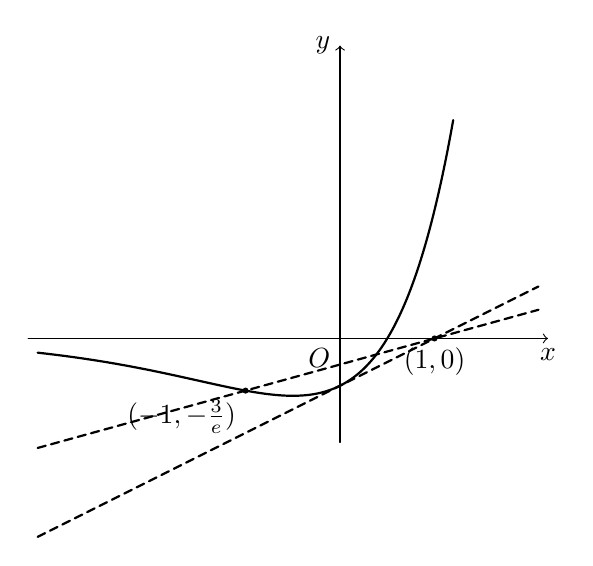
\begin{tikzpicture}[x=1.2cm,y=0.6cm,line cap=round,line join=round]
  \draw[->] (-3.3,0) -- (2.2,0) node[below] {$x$};
  \draw[->] (0,-2.2) -- (0,6.2) node[left] {$y$};
  \node[below left] at (0,0) {$O$};

  % 曲线 y=e^x(2x-1)
  \draw[thick,smooth,samples=220,domain=-3.2:1.2]
    plot (\x,{exp(\x)*(2*\x-1)});

  % 第一条虚线：y=x-1（题图里那条“切线”示意）
  \draw[densely dashed,thick] (-3.2,{-3.2-1}) -- (2.1,{2.1-1});

  % 点 (-1,-3/e) 与 (1,0)
  \pgfmathsetmacro{\yB}{-3/exp(1)} % -3/e
  \fill (-1,\yB) circle (1.1pt);
  \node[below left] at (-1,\yB) {$(-1,-\frac{3}{e})$};

  \fill (1,0) circle (1.1pt);
  \node[below] at (1,0) {$(1,0)$};

  % 第二条虚线：过 (1,0) 与 (-1,-3/e)
  % 斜率 m = (0-(-3/e))/(1-(-1)) = 3/(2e)
  % 方程 y = (3/(2e))(x-1)
  \pgfmathsetmacro{\m}{3/(2*exp(1))}
  \draw[densely dashed,thick]
    (-3.2,{\m*(-3.2-1)}) -- (2.1,{\m*(2.1-1)});
\end{tikzpicture}

由 $ y'\big|_{x=0}=1 $ 可得 $ y=e^x(2x-1) $ 在 $ (0,-1) $ 处的切线方程为 $ y=x-1 $，观察图像可知 $ a=1 $ 就是一个临界情形；

当 $ a $ 从 $ 1 $ 逐渐变小时，$ y=ax-a $ 绕点 $ (-1,0) $ 顺时针旋转，考虑点 $ \left(-1,-\dfrac{3}{e}\right) $ 在 $ y=e^x(2x-1) $ 上，当 $ y=ax-a $ 经过 $ \left(-1,-\dfrac{3}{e}\right) $ 即 $ a=\dfrac{3}{2e} $ 时，这是另一个临界情形，如果 $ a $ 继续变小，那么 $ y=e^x(2x-1) $ 就有 $ (0,-1) $，$ \left(-1,-\dfrac{3}{e}\right) $ 两个横坐标为整数的点位于 $ y=ax-a $ 下方，不满足题意，综上选 D.
\end{solutions}